\documentclass[a4paper,12pt,titlepage,finall]{article}

\usepackage[T1,T2A]{fontenc}     % форматы шрифтов
\usepackage[utf8]{inputenc}      % кодировка символов, используемая в данном файле
\usepackage[english, russian]{babel}      % пакет русификации
\usepackage{tikz}                % для создания иллюстраций
\usepackage{pgfplots}            % для вывода графиков функций
\usepackage{geometry}		     % для настройки размера полей
\usepackage{indentfirst}         % для отступа в первом абзаце секции
\usepackage{amsmath,amsthm,amssymb}
\usepackage{mathtext}
\usepackage{graphicx}

\usepackage{caption}
\usepackage{subcaption}
\usepackage{hyperref}
\graphicspath{ {./img} }

%Настройка листингов для языка C
\usepackage{xcolor}
\usepackage{listings}
\lstset{extendedchars=\true}

\definecolor{mGreen}{rgb}{0,0.6,0}
\definecolor{mGray}{rgb}{0.5,0.5,0.5}
\definecolor{mPurple}{rgb}{0.58,0,0.82}
\definecolor{backgroundColour}{rgb}{0.95,0.95,0.95}

\lstdefinestyle{CStyle}{
    backgroundcolor=\color{backgroundColour},   
    keywordstyle=\color{mGreen},
    numberstyle=\tiny\color{mGray},
    breakatwhitespace=false,         
    breaklines=true,                 
    captionpos=b,                    
    keepspaces=true,                 
    numbers=none,                    
    numbersep=5pt,                  
    showspaces=false,                
    showstringspaces=false,
    showtabs=false,                  
    tabsize=2,
    language=C,
    basicstyle=\footnotesize\ttfamily ,
    extendedchars=\true ,
}

% выбираем размер листа А4, все поля ставим по 3см
\geometry{a4paper,left=30mm,top=30mm,bottom=30mm,right=30mm}

\setcounter{secnumdepth}{0}      % отключаем нумерацию секций
\setcounter{tocdepth}{2}

\usepgfplotslibrary{fillbetween} % для изображения областей на графиках

\begin{document}
\begin{titlepage}
    \begin{center}
	{\small \sc Московский государственный университет \\имени М.~В.~Ломоносова\\
	Факультет вычислительной математики и кибернетики\\}
	\hrulefill
	\vfill
	{\large \bf Компьютерный практикум по учебному курсу}\\
	~\\
	{\Large \bf <<ВВЕДЕНИЕ В ЧИСЛЕННЫЕ МЕТОДЫ>>}\\ 
	~\\
	~\\
	~\\
	{\Large \bf ЗАДАНИЕ № 2}\\
	~\\
	{\bf Численные методы решения дифференциальных уравнений}\\
	~\\
	{\large \bf ОТЧЕТ}\\
	{\bf о выполненном задании}\\
	{студента 201 учебной группы факультета ВМК МГУ}\\
	{Галустова Артемия Львовича}
    \end{center}
    
    \begin{center}
	\vfill
	{\small гор. Москва\\2020 год}
    \end{center}
\end{titlepage}

\tableofcontents
\newpage
\section{Подвариант 1}
\subsection{Цель работы}
Освоить методы Рунге-Кутты второго и четвертого порядка точности,
применяемые для численного решения задачи Коши для дифференциального
уравнения (или системы дифференциальных уравнений) первого порядка.

\subsection{Постановка задачи}
Рассматривается обыкновенное дифференциальное уравнение первого порядка,
разрешенное относительно производной и имеющее вид:
\begin{align*}
\frac{dy}{dx}=f(x,y), x_0 < x,
\end{align*}

с дополнительным начальным условием, заданным в точке $x = x_0$ :
\begin{align*}
y(x_0)=y_0.
\end{align*}

Предполагается, что  функция $f = f (x, y)$ такова, что
гарантирует существование и единственность решения задачи Коши.
В том случае, если рассматривается не одно дифференциальное уравнение, а система обыкновенных дифференциальных уравнений первого порядка,
разрешенных
относительно
производных
неизвестных
функций, то
соответствующая задача Коши имеет вид (на примере двух дифференциальных
уравнений):
\begin{align*}
\begin{cases}
\frac{dx}{dt}=f_1(t,x,y),\\
\frac{dy}{dt}=f_2(t,x,y),
\end{cases}
\end{align*}
\par
Дополнительные (начальные) условия задаются в точке $x = x_0$:
\begin{align*}
x(t_0) = x_0, y(t_0)=y_0.
\end{align*}

Также предполагается, что $f_1, f_2$ заданы так, что это
гарантирует существование и единственность решения задачи Коши, но
уже для системы обыкновенных дифференциальных уравнений первого порядка в
форме, разрешенной относительно производных неизвестных функций.
\par
Требуется найти численное решение для данных задач Коши.

\subsection{Цели и задачи практической работы}
\begin{enumerate}
\item
Решить задачу Коши наиболее известными и широко
используемыми на практике методами Рунге-Кутта второго и четвертого
порядка
точности,
аппроксимировав
дифференциальную
задачу
соответствующей разностной схемой (на равномерной сетке); полученное
конечно-разностное уравнение (или уравнения в случае системы),
представляющее фактически некоторую рекуррентную формулу, просчитать
численно;
\item
Найти численное решение задачи и построить его график;
\item
Найденное численное решение сравнить с точным решением
дифференциального уравнения (подобрать специальные тесты, где
аналитические решения находятся в классе элементарных функций, для проверки и построения графиков использован онлайн сервис символьных вычислений Wolfaram One).

\end{enumerate}
\newpage
\subsection{Описание метода решения}
\subsubsection{Метод Рунге-Кутты для обыкновенного дифференциального уравнения первого порядка разрешённого относительно производной}
Пусть дано обыкновенное дифференциальное уравнение первого порядка разрешённое относительно производной на отрезке $[x_0, x_0 + l], l > 0$:
\begin{align*}
y'(x)=f(x,y(x)), x \in [x_0, x_0 + l]
\end{align*}
Рассмотрим сетку равномерную сетку $x_i = x_0 + ih, i = 0, 1, 2 ... n, h = \frac{l}{n}$. Где $n$ - число шагов и является параметром алгоритма. Также обозначим $y_i = y(x_i)$. Метод Рунге-Кутты второго порядка точности задаёт рекуррентную формулу
\begin{align*}
&k_1 = f(x_i, y_i)\\
&k_2 = f(x_i + h, y_i + h * k_1)\\
&y_{i + 1} = y_i + \frac{h}{2}(k_1 + k_2).
\end{align*} 
\par
Метод четвёртого порядка точности задаёт рекуррентную формулу
\begin{align*}
y_{i+1} = \frac{h}{6} (k_1 +2k_2 + 2k_3 + k_4)
\end{align*}
где
\begin{align*}
&k_1 = f(x_i, y_i)\\
&k_2 = f(x_i + \frac{h}{2}, y_i + \frac{h}{2}k_1)\\
&k_3 = f(x_i + \frac{h}{2}, y_i + \frac{h}{2}k_2)\\
&k_4 = f(x_i + h, y_i + hk_3)
\end{align*}

\subsubsection{Метод Рунге-Кутты для системы двух обыкновенных дифференциальных уравнений первого порядка разрешённых относительно производной}
Пусть дана систем двух обыкновенных дифференциальных уравнений первого порядка разрешённых относительно производной на отрезке $[t_0, t_0 + l], l > 0$:
\begin{align*}
\begin{cases}
x'(t)=f_1(t,x,y)\\
y'(t)=f_2(t,x,y)
\end{cases}
\end{align*}
Рассмотрим сетку равномерную сетку $t_i = t_0 + ih, i = 0, 1, 2 ... n, h = \frac{l}{n}$. Где $n$ - число шагов и является параметром алгоритма. Метод Рунге-Кутты второго порядка точности для системы аналогичен таковому для одного уравнения и задаёт рекуррентную формулу
\begin{align*}
x_{i+1} = x_i + \frac{h}{2}(k_1 + k_2)\\
y_{i+1} = y_i + \frac{h}{2}(l_1 + l_2)
\end{align*}
где
\begin{align*}
&k_1 = f_1(t_i, x_i, y_i),~~ l_1 = f_2(t_i, x_i, y_i)\\
&k_2 = f_1(t_i + h, x_i + h k_1, y_i + h l_1),~~ l_2 = f_2(t_i + h, x_i + h k_1, y_i + h l_1)\\
\end{align*}
Метод четвёртого порядка точности задаёт рекуррентную формулу
\begin{align*}
x_{i+1} = x_i + \frac{h}{6}(k_1 + 2 k_2 + 2 k_3 + k_4)\\
y_{i+1} = y_i + \frac{h}{6}(l_1 + 2 l_2 + 2 l_3 + l_4)
\end{align*}
где
\begin{align*}
&k_1 = f_1(t_i, x_i, y_i), ~~ l_1 = f_2(t_i, x_i, y_i)\\
&k_2 = f_1(t_i + \frac{h}{2}, x_i + \frac{h}{2}k_1, y_i + \frac{h}{2}l_1), ~~ l_2 = f_2(t_i + \frac{h}{2}, x_i + \frac{h}{2}k_1, y_i + \frac{h}{2}l_1)\\
&k_3 = f_1(t_i + \frac{h}{2}, x_i + \frac{h}{2}k_2, y_i + \frac{h}{2}l_2), ~~ l_3 = f_2(t_i + \frac{h}{2}, x_i + \frac{h}{2}k_2, y_i + \frac{h}{2}l_2)\\
&k_4 = f_1(t_i + h, x_i + h k_3, y_i + h l_3), ~~ l_4 = f_2(t_i + h, x_i + h k_3, y_i + h l_3)
\end{align*}
\newpage
\subsection{Описание программы}
Данный алгоритм был реализован на языке С с применением стандартной библиотеки языка С. Ниже приведена часть файла RK.c содержащая реализацию описанных выше методов. Полный код программы доступен в разделе <<\nameref{source}>>, а также онлайн по адресу \url{https://github.com/NotLebedev/de_solver}.
\lstinputlisting[style=CStyle, firstline=5]{../RK.c}

\subsection{Тестирование}
Для проверки результатов выполнения программы на тестах был использован использован онлайн сервис символьных вычислений Wolfaram One. Были подобраны примеры с аналитическим решением, и построены графики их решений с наложением точек полученных в результате работы программы. Были проведены тесты для числа шагов $n = 10, 100, 1000$, а также для второго и четвёртого порядка точности.
\begin{enumerate}
\item
Уравнение $y'(x) = -\frac{y}{x}$ с начальными условиями $y(1)=3$. Аналитическое решение $y = \frac{3}{x}$.
\begin{figure}[h]
\centering
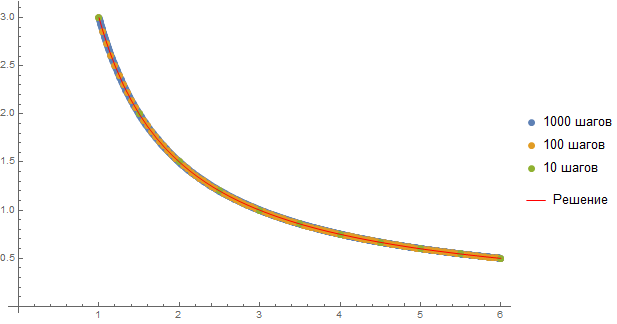
\includegraphics[width=0.7\textwidth]{test_1_1_2.png}
\caption{Второй порядок точности}
\centering
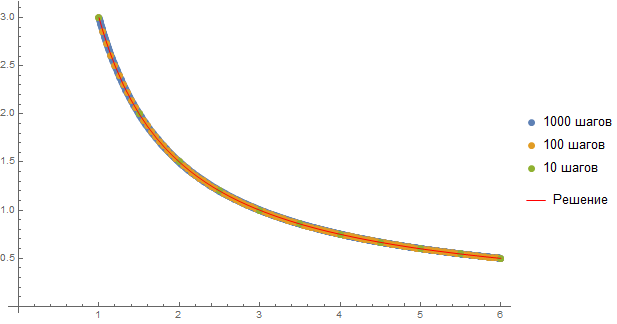
\includegraphics[width=0.7\textwidth]{test_1_1_4.png}
\caption{Четвёртый порядок точности}
\end{figure}
\par
Численное решения при любой точности метода и любом числе шагов близко к аналитическому.

\newpage
\item
Уравнение $y'(x) = 3x sin(x) - y$ с начальными условиями $y(0)=2$. Аналитическое решение $y = \frac{1}{2} (e^{-x} - 3 (-1 + x) \cos (x) + 3 x \sin (x))$.
\begin{figure}[h]
\centering
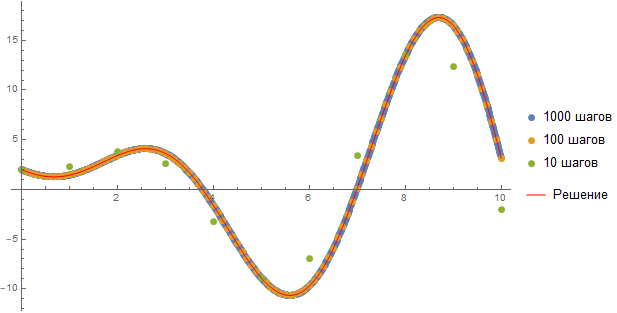
\includegraphics[width=0.7\textwidth]{test_1_2_2.png}
\caption{Второй порядок точности}
\centering
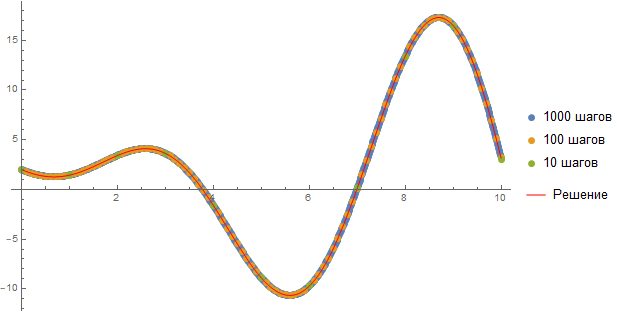
\includegraphics[width=0.7\textwidth]{test_1_2_4.png}
\caption{Четвёртый порядок точности}
\end{figure}
\par
Численное решения при использовании второго порядка точности и малого числа шагов существенно отличается от аналитического. При использовании четвёртого порядка точности даже при $n = 10$ решение близко к аналитическому.

\newpage
\item
Уравнение $y'(x) = x^2 y + x^2$ с начальными условиями $y(-2)=-2$. Аналитическое решение $y = -1 -e^{\frac{1}{3}(x^3 + 8)}$.
\begin{figure}[h]
\centering
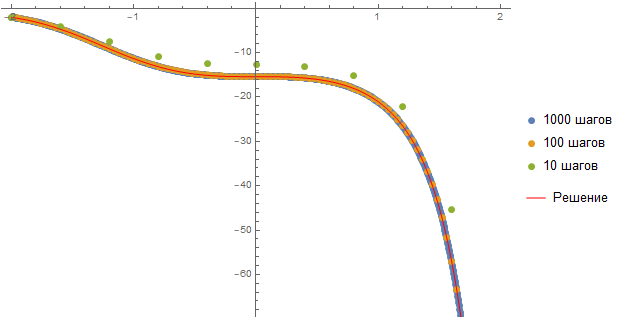
\includegraphics[width=0.7\textwidth]{test_1_3_2.png}
\caption{Второй порядок точности}
\centering
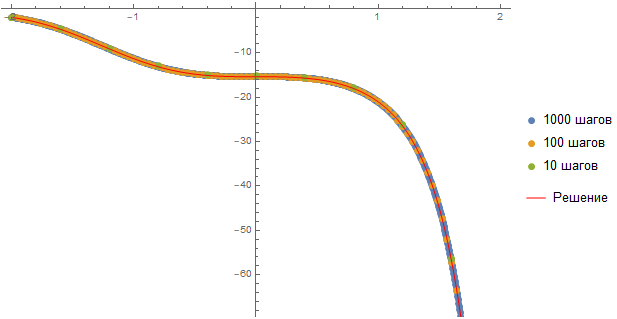
\includegraphics[width=0.7\textwidth]{test_1_3_4.png}
\caption{Четвёртый порядок точности}
\end{figure}

\newpage
\item
Уравнение $y'(x) = (y - y^2) x$ с начальными условиями $y(0)= 3$. Аналитическое решение $y = \left( 1- \frac{2}{3} e^{-\frac{1}{2}x^2} \right)^{-1}$.
\begin{figure}[h]
\centering
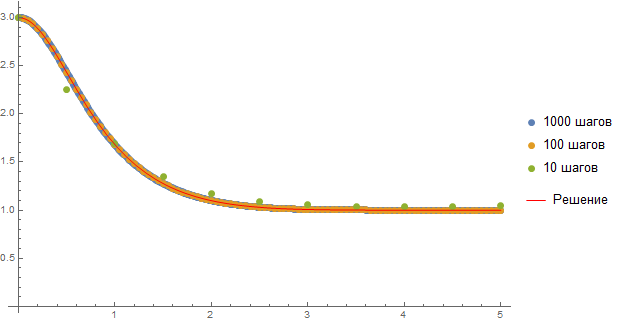
\includegraphics[width=0.7\textwidth]{test_1_4_2.png}
\caption{Второй порядок точности}
\centering
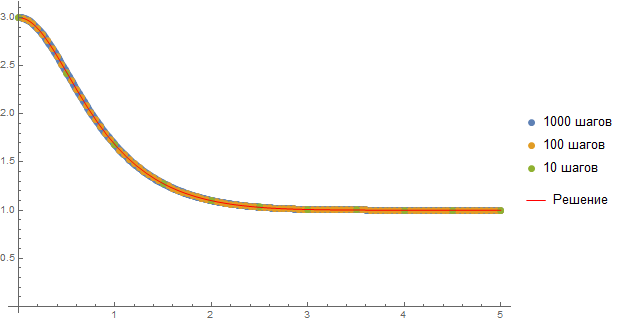
\includegraphics[width=0.7\textwidth]{test_1_4_4.png}
\caption{Четвёртый порядок точности}
\end{figure}

\newpage
\item
Система $x' = -x -5y, y' = x + y$ с начальными условиями $x(0) = 2, y(0)= 3$. Аналитическое решение $x = 2 \cos (2 t) - 17 \cos (t) \sin(t), y = 3 \cos (2 t) + 5 \cos (t) \sin (t)$.
\begin{figure}[h]
\centering
\begin{subfigure}{.5\textwidth}
  \centering
  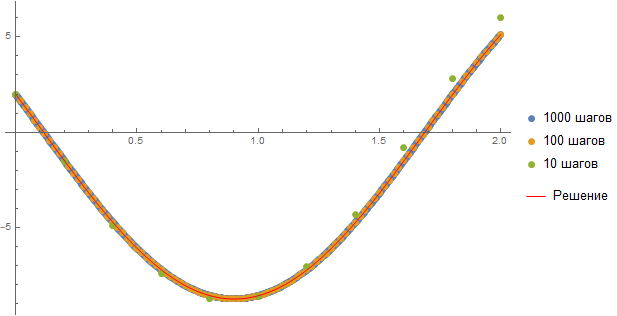
\includegraphics[width=\textwidth]{test_1_5_2_x.png}
\end{subfigure}%
\begin{subfigure}{.5\textwidth}
  \centering
  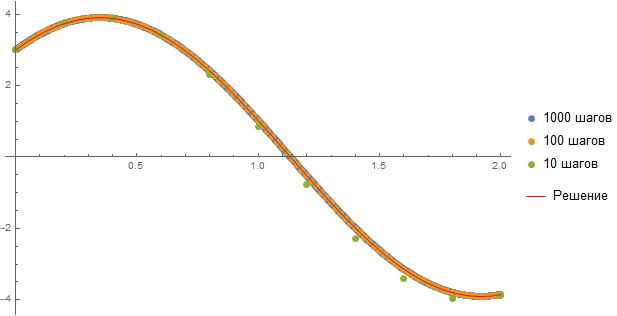
\includegraphics[width=\textwidth]{test_1_5_2_y.png}
\end{subfigure}
\caption{Второй порядок точности, графики $x(t)$ и $y(t)$ соответственно}
\centering
\begin{subfigure}{.5\textwidth}
  \centering
  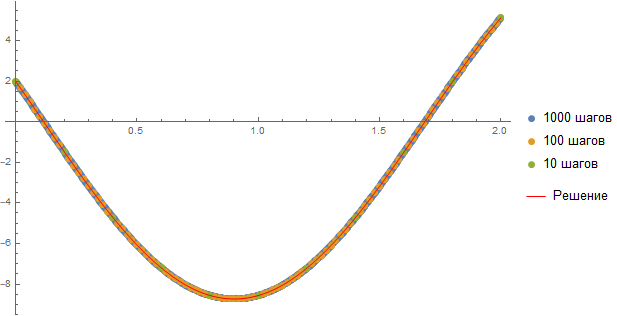
\includegraphics[width=\textwidth]{test_1_5_4_x.png}
\end{subfigure}%
\begin{subfigure}{.5\textwidth}
  \centering
  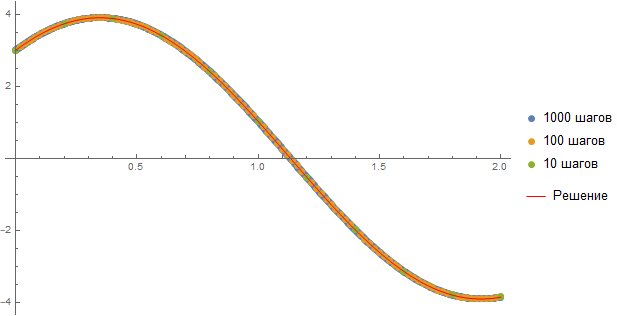
\includegraphics[width=\textwidth]{test_1_5_4_y.png}
\end{subfigure}
\caption{Четвёртый порядок точности, графики $x(t)$ и $y(t)$ соответственно}
\end{figure}
\par
Видно, что точность метода для системы уравнений сходна с точностью для одиночного уравнения. Метод второго порядка точности даёт численное решение существенно отличающееся от аналитического, в то время, как метод четвёртого порядка даже при $n=10$ даёт весьма точный результат.

\newpage
\item
Система $x' = 4x + y - e^{2t}, y' = y - 2x$ с начальными условиями $x(0) = 1, y(0)= -1$. Аналитическое решение $x = e^{2 t} (2 - e^t + t), y = e^{2 t} (e^t - 2 (1 + t))$.
\begin{figure}[h]
\centering
\begin{subfigure}{.5\textwidth}
  \centering
  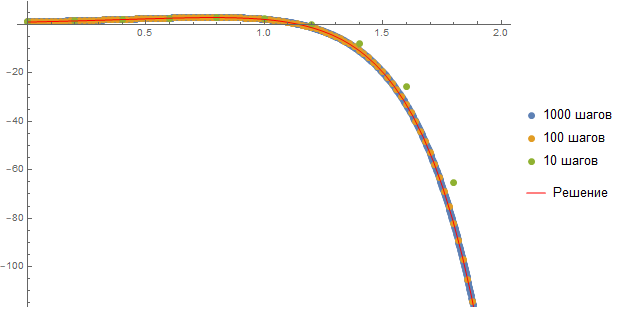
\includegraphics[width=\textwidth]{test_1_6_2_x.png}
\end{subfigure}%
\begin{subfigure}{.5\textwidth}
  \centering
  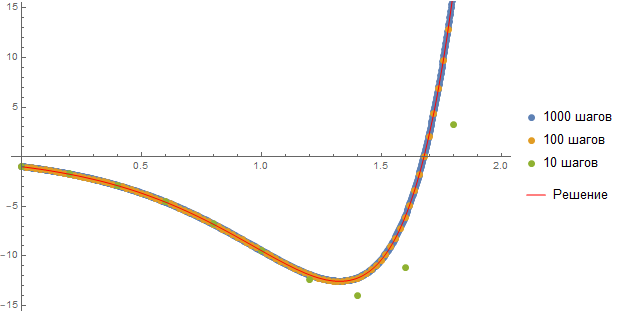
\includegraphics[width=\textwidth]{test_1_6_2_y.png}
\end{subfigure}
\caption{Второй порядок точности, графики $x(t)$ и $y(t)$ соответственно}
\centering
\begin{subfigure}{.5\textwidth}
  \centering
  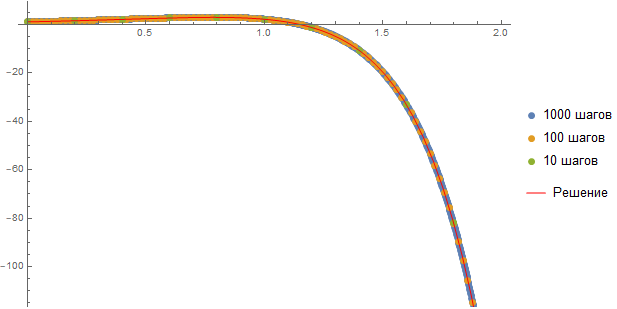
\includegraphics[width=\textwidth]{test_1_6_4_x.png}
\end{subfigure}%
\begin{subfigure}{.5\textwidth}
  \centering
  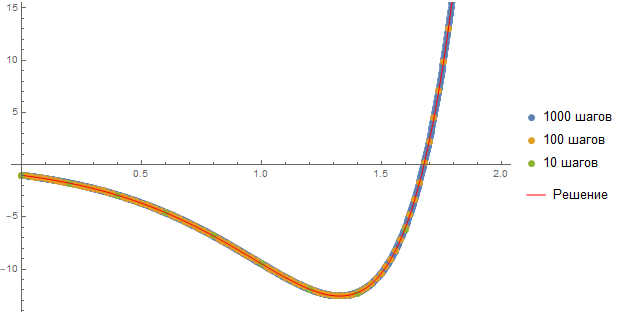
\includegraphics[width=\textwidth]{test_1_6_4_y.png}
\end{subfigure}
\caption{Четвёртый порядок точности, графики $x(t)$ и $y(t)$ соответственно}
\end{figure}

\newpage
\item
Система $x' = t + x - y^2 +2, y' = \sin(t - x) + 2,1 y$ с начальными условиями $x(0) = 1.5, y(0)= 0$. Аналитическое решение найти не удалось.
\begin{figure}[h]
\centering
\begin{subfigure}{.5\textwidth}
  \centering
  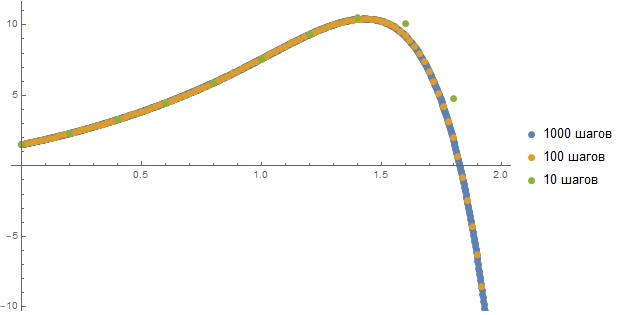
\includegraphics[width=\textwidth]{test_1_7_2_x.png}
\end{subfigure}%
\begin{subfigure}{.5\textwidth}
  \centering
  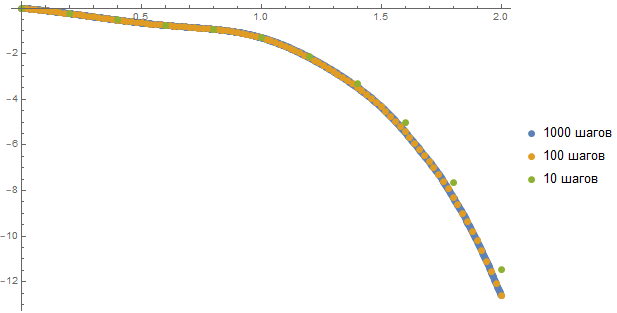
\includegraphics[width=\textwidth]{test_1_7_2_y.png}
\end{subfigure}
\caption{Второй порядок точности, графики $x(t)$ и $y(t)$ соответственно}
\centering
\begin{subfigure}{.5\textwidth}
  \centering
  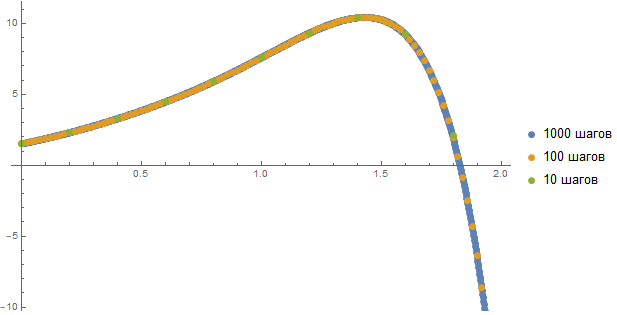
\includegraphics[width=\textwidth]{test_1_7_4_x.png}
\end{subfigure}%
\begin{subfigure}{.5\textwidth}
  \centering
  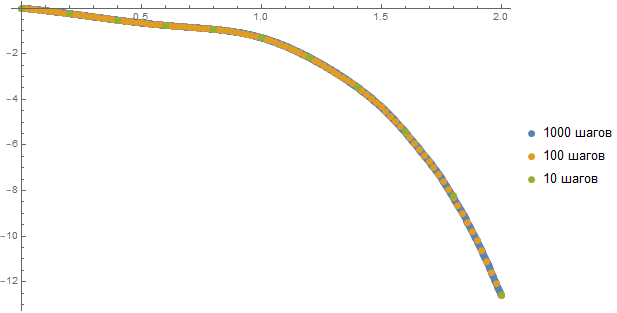
\includegraphics[width=\textwidth]{test_1_7_4_y.png}
\end{subfigure}
\caption{Четвёртый порядок точности, графики $x(t)$ и $y(t)$ соответственно}
\end{figure}
\end{enumerate}
\subsection{Выводы}
При выполнении поставленных целей был подробно разобран и реализован метод Метод Рунге-Кутты второго и четвёртого порядка точности для уравнений и систем. Метод второго порядка точности прост для реализации и удобен для вычислений, однако может иметь большие погрешности вычислений при малом числе точек. Метод четвёртого порядка существенно меньше подвержен этой проблеме, что оправдывает увеличенную сложность алгоритма и дополнительные вычисления на каждом шаге.

\newpage
\section{Подвариант 1}
\subsection{Цель работы}
Освоить метод прогонки решения краевой задачи для дифференциального
уравнения второго порядка.

\subsection{Постановка задачи}
Рассматривается линейное дифференциальное уравнение вида
\begin{align*}
y''(x) + p(x) y'(x) + q(x) y(x) = f(x), x_0 < x < x_n  
\end{align*}
с дополнительными условиями в граничных точках
\begin{align*}
&\sigma_1 y(x_0) + \gamma_1 y'(x_0) = \delta_1\\
&\sigma_2 y(x_n) + \gamma_2 y'(x_n) = \delta_2
\end{align*}

\subsection{Цели и задачи практической работы}
\begin{enumerate}
\item
Решить данную краевую задачу методом конечных разностей, аппроксимировав ее разностной схемой второго порядка точности (на равномерной сетке); полученную систему конечно-разностных уравнений решить методом прогонки;
\item
Найти разностное решение задачи и построить его график;
\item
Найденное разностное решение сравнить с точным решением
подобрать специальные тесты, где
аналитические решения находятся в классе элементарных функций, для проверки и построения графиков использован онлайн сервис символьных вычислений Wolfaram One).
\end{enumerate}

\newpage
\subsection{Описание метода решения}
Рассмотрим линейное дифференциальное уравнение с начальными условиями в граничных точках второго порядка на отрезке $[x_0, x_n]$
\begin{align*}
&y''(x) + p(x) y'(x) + q(x) y(x) = f(x), x_0 < x < x_n \\
&\sigma_1 y(x_0) + \gamma_1 y'(x_0) = \delta_1\\
&\sigma_2 y(x_n) + \gamma_2 y'(x_n) = \delta_2
\end{align*}
Рассмотрим равномерную сетку $x_i = x_0 + ih, i = 0, 1, 2 ... n, h = \frac{x_n - x_0}{n}$, где $n$ - число шагов и является параметром алгоритма. Также обозначим $y_i = y(x_i)$. Аппроксимируем производные в исходном уравнении конечно-разностными отношениями второго порядка точности:
\begin{align*}
&\frac{y_{i+1} - 2y_i + y_{i-1}}{h^2} + p(x_i) \frac{y_{i+1} - y_{i-1}}{2h} + q(x_i) y_i = f(x_i), 1 \leq i \leq n - 1\\
&y_{i+1} \left( \frac{1}{h^2} + \frac{p(x_i)}{2h} \right) + y_i \left( -\frac{2}{h^2} + q(x_i) \right) + y_{i-1} \left( \frac{1}{h^2} - \frac{p(x_i)}{2h} \right) = f(x_i)
\end{align*}

Также аппроксимируем производные в граничных условиях кончено-разностными отношениями первого порядка точности:
\begin{align*}
&\sigma_1 y_0 + \gamma_1 \frac{y_1 - y_0}{h} = \delta_1\\
&y_0 \left( \sigma_1  - \frac{\gamma_1}{h} \right) + y_1 \frac{\gamma_1}{h} = \delta_1\\
&\\
&\sigma_2 y_n + \gamma_2 \frac{y_n - y_{n-1}}{h} = \delta_2\\
&y_n \left( \sigma_2  + \frac{\gamma_2}{h} \right) - y_{n-1} \frac{\gamma_2}{h} = \delta_2
\end{align*}

Итого имеется система из $n+1$ уравнения с $n+1$ неизвестной, с матрицей трёхдиагональной матрицей. Эта система может быть решена методом прогонки, решение ищется в виде $y_i = \alpha_{i+1} x_{i+1} + \beta_{i+1}, i = n-1, n-2 .. 1$. Коэффициенты матрицы имеют вид $A_i = \frac{1}{h^2} - \frac{p(x_i)}{2h}, B_i = -\frac{2}{h^2} + q(x_i), C_i = \frac{1}{h^2} + \frac{p(x_i)}{2h}, i = 1, .. n -1$. Тогда прогоночные коэффициенты $\alpha_{i+1} = \frac{-C_i}{A_i \alpha_i + B_i}, \beta_{i+1} = \frac{F_i - A_i \beta_i}{A_i \alpha_i + B_i}$. Из граничных условий также получаем $\alpha_0 = \frac{\gamma_1}{\sigma_1 * h - \gamma_1}, \beta_0 = \frac{\delta_1}{\sigma_1 - \frac{\gamma_1}{h}}$, а величина $y_i$ для $i = n$ имеет вид $y_n = \frac{\delta_2 h + \gamma_2 \beta_{n-1}}{\sigma_2 h + \gamma_2 - \gamma_2 \alpha_{n-1}}$.

\newpage
\subsection{Описание программы}
Данный алгоритм был реализован на языке С с применением стандартной библиотеки языка С. Ниже приведена часть файла RK.c содержащая реализацию описанных выше методов. Полный код программы доступен в разделе <<\nameref{source}>>, а также онлайн по адресу \url{https://github.com/NotLebedev/de_solver}.
\lstinputlisting[style=CStyle, firstline=4]{../boundary.c}

\newpage
\subsection{Тестирование}
\begin{enumerate}
\item
Уравнение $y'' - \frac{6y}{x^2} = 0$ с начальными условиями $y(0) = 0, y'(1) - y(1) = 1$. Аналитическое решение $y = \frac{x^3}{2}$.
\begin{figure}[h]
\centering
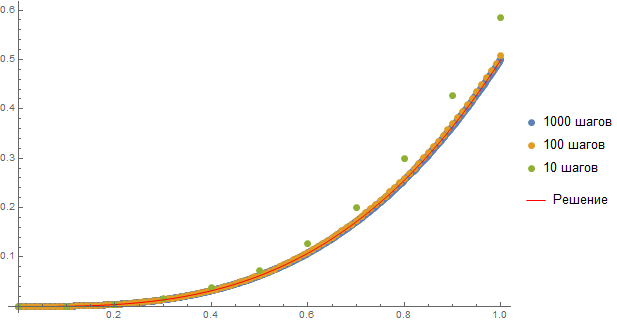
\includegraphics[width=0.7\textwidth]{test_2_1.png}
\end{figure}
\par
Точность численного решения зависит от числа шагов и даже при $n = 100$ отличается от аналитического.

\item
Уравнение $y'' - 2y' + y = e^x$ с начальными условиями $y(0) = 1, y'(1) = 1$. Аналитическое решение $y = \frac{1}{4} e^{x} (\frac{2}{e} x + (4 - 5 x + 2 x^2))$.
\begin{figure}[h]
\centering
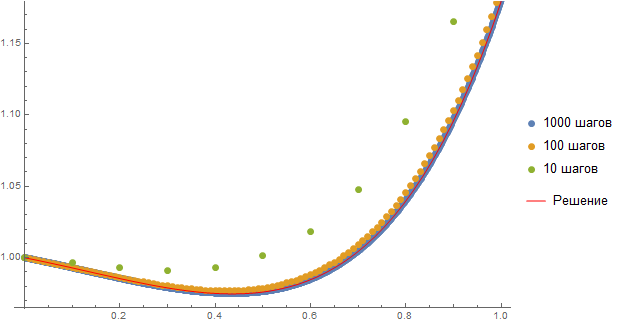
\includegraphics[width=0.7\textwidth]{test_2_2.png}
\end{figure}
\par
Точность численного решения зависит от числа шагов и погрешность при малом числе шагов ещё более существенна чем в предыдущем примере.
\newpage
\item
Уравнение $y'' - y = \frac{1}{x} - \frac{2}{x^3}$ с начальными условиями $y'(2) = 0,25, y(5) + y'(5) = -0.16$. Аналитическое решение $y = -\frac{1}{x}$.
\begin{figure}[h]
\centering
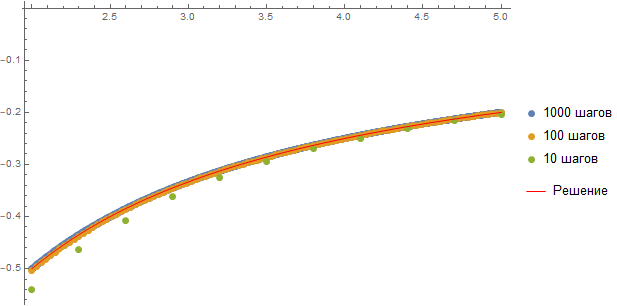
\includegraphics[width=0.7\textwidth]{test_2_3.png}
\end{figure}
\par
Точность численного решения зависит от числа шагов, но сходимость лучше чем в предыдущих примерах.
\end{enumerate}
\end{document}